\documentclass{article}

% if you need to pass options to natbib, use, e.g.:
%     \PassOptionsToPackage{numbers, compress}{natbib}
% before loading neurips_2020

% ready for submission
% \usepackage{neurips_2020}

% to compile a preprint version, e.g., for submission to arXiv, add add the
% [preprint] option:
%     \usepackage[preprint]{neurips_2020}

% to compile a camera-ready version, add the [final] option, e.g.:
%     \usepackage[final]{neurips_2020}

% to avoid loading the natbib package, add option nonatbib:
\usepackage{neurips_2020}

\usepackage[utf8]{inputenc} % allow utf-8 input
\usepackage[T1]{fontenc}    % use 8-bit T1 fonts
\usepackage{hyperref}       % hyperlinks
\usepackage{url}            % simple URL typesetting
\usepackage{booktabs}       % professional-quality tables
\usepackage{amsfonts}       % blackboard math symbols
\usepackage{nicefrac}       % compact symbols for 1/2, etc.
\usepackage{xcolor}
\usepackage{ulem}

\usepackage{microtype}      % microtypography
\usepackage{amsmath}
\usepackage{graphicx}
\usepackage{arydshln}

\newcommand{\Edouard}[1]{\textcolor{blue}{#1}}
\newcommand{\mynotes}[1]{\textcolor{red}{#1}}
\title{On the Role of Patches in \Edouard{ Analysis of}  Image Classification \Edouard{models}}


% The \author macro works with any number of authors. There are two commands
% used to separate the names and addresses of multiple authors: \And and \AND.
%
% Using \And between authors leaves it to LaTeX to determine where to break the
% lines. Using \AND forces a line break at that point. So, if LaTeX puts 3 of 4
% authors names on the first line, and the last on the second line, try using
% \AND instead of \And before the third author name.

\author{%
  David S.~Hippocampus\thanks{Use footnote for providing further information
    about author (webpage, alternative address)---\emph{not} for acknowledging
    funding agencies.} \\
  Department of Computer Science\\
  Cranberry-Lemon University\\
  Pittsburgh, PA 15213 \\
  \texttt{hippo@cs.cranberry-lemon.edu} \\
  % examples of more authors
  % \And
  % Coauthor \\
  % Affiliation \\
  % Address \\
  % \texttt{email} \\
  % \AND
  % Coauthor \\
  % Affiliation \\
  % Address \\
  % \texttt{email} \\
  % \And
  % Coauthor \\
  % Affiliation \\
  % Address \\
  % \texttt{email} \\
  \And
  Edouard Oyallon \\
  CNRS/LIP6 \\
  Sorbonne University \\
  \texttt{edouard.oyallon@lip6.fr} \\
}

\begin{document}

\maketitle

\begin{abstract}
  Several recent work towards understanding deep learning and building more principled deep learning models have focused on constructing models for the image classification setting. These models typically share aspects of deep convolutional networks used in practice while being more amenable to theoretical analysis. Although the performance gap of these models has decreased one can observe they all share as a typical preprocessing step the extraction of features based on random patches from natural images. Although characterized as a non-critical step, in this work we investigate the role of this patch based feature extraction finding that it is the primary driver of high performance. Indeed we observe that one can recover XX \% on the CIFAR-10 dataset using just a method which matches patches in an image to nearest neighbors. Subsequently we ask what is hte limit of such an approach on a large scale dataset such as imagenet, finding that it can obtain performance compatible to methods relying on sophisticated image processign algorithm
 
\end{abstract}

\section{Introduction}
% this paragraph must motivate why image classification analysis is difficult and the fact  that performance is one of the criterium used by researchers, that should be on imagenet - I think now it's good and clear
Understanding the success of deep convolutional neural networks on images has received a plethora of interest from the machine learning community. 
This is challenging because images are high-dimensional signals and deep neural networks are highly-non linear models  with a substantial amount of parameters: the curse of dimensionality is seemingly avoided by these models. These analysis are thus difficult, and  their final conclusions are often relayed to obtaining  good  performances on standard benchmarks. Furthermore, there  exists generally a substential gap  of performances between the numerical experiments of works based on theorertical considerations and heavily engineered pipelines \citep{krizhevsky2012imagenet}. Several recent works have aimed to close this gap, attempting to provide models that have approachable theoretical properties but still providing a high performance
~\citep{li2019enhanced,shankar2020neural}. Yet, in general, they lack of large scale experiments on datasets such as ImageNet.



% This paragraph must discuss a/ the fact that a lot of theoretical(eg arora)/empirical(eg bagnet) works are implicitely or explicitely patch based b/ They don't do the necessary ablations to see that and the low dimensional structure of patches is quite more reasonable idea
Our work is primarly motivated by the emergent principle that  deep learning success  could be reproduced by   designing appropriate kernels \citep{mairal2016end,li2019enhanced,shankar2020neural,lu2014scale}, which have favorable theoretical properties~\citep{jacot2018neural,rahimi2008random}. We aim to show that  the those vision works rely on patch extraction and this latter is implicitely the key of their success.  Indeed, without ablation experiments, it is difficult to know which of  the correct modeling of the problem or  the ad-hoc engeneering choices is important. We argue that those works can be in fact understood through the common  lense of representations constituted by a single dictionary of patches: we decompose and analyze each step of our feature design, on gold-standard  datasets. We further note that this idea is aligned with empirical studies that relate the models decisions with visual interpretations at small and large patch level
\citep{zeiler2014visualizing,brendel2019approximating}, which suggests that the intrinsic dimension of patches is quite  lower than the original signal's dimension and they are easier to interpret.



We remind well-known properties of patches. By construction,  they are locally stationnary processus obtained from images, and it can be empirically verified that they are sparsified in a wavelet basis~\citep{mallat1999wavelet}. Furthermore, they are often the very first component of many classic vision pipelines \citep{perronnin2010improving,lowe2004distinctive,brendel2019approximating,oyallon2018scattering}. While one has a good understanding of the behavior of a dictionary of patches for image compression
~\citep{wallace1992jpeg}, texture synthesis~\citep{efros1999texture} or image inpainting ~\citep{criminisi2004region} , we have a limited knowledge and understanding of it in the context of image classification. We address this is issue by studying this experimentally.

One of our major contribution is to introduce a representation that does not involve learning (up to a linear classifier) and to our knowledge, it outperforms by a large margin the classification accuracy of former attempts to get rid of representation learning on the large-scale ImageNet dataset. Our representation is based on a dictionary of whitened patches: pair-wise distances between this dictionary and the patches of each images are computed, quantized and then fed to a linear classifier. This method is  straightforward and involves a limited ad-hoc feature engineering. \Edouard{Note that other papers which work at the patch level can be understood as linear embeddings that rely on some Euclidean distances between patches: our results indicate that a Hamming distance between well-chosen set of patches is a surprisingly good baseline.} As discussed in Section \ref{related_work}, we believe that we are the first line of work to explicitly show that this  spare feature is solely achieving non-trivial performances on difficult datasets.

% Structure of the paper
Our paper is structured as follow: first, we discuss the related works (Sec.~\ref{related_work}). Then, Sec.~\ref{method} explain precisely how our visual representation is built. In Sec.~\ref{experiments}, we present experimental results on the vision datasets CIFAR-10 and the large scale  ImageNet as well as a collection of numerical experiments to disentangle the different components of our model. At the time of publication, we will release our code online as well as the commands to reproduce exactly our results.


\section{Related work}
\label{related_work}

The seminal works \cite{coates2011analysis} and \cite{coates2011importance}  study patch-based representations on CIFAR-10.
They set the first baseline for a single-layer convolutional neural network initialized with random patches, and they show it  can achieve a non-trivial performance ($\sim 80 \%$) on the CIFAR-10 dataset. However, they lack two key ingredients: the scale (e.g., no ImageNet, few patches) and the classification procedure (e.g., no data augmentation).
 \cite{recht2019imagenet} published an implementation of this technique and conducted large scale experiments with hundreds of thousands of random patches, improving the accuracy ($\sim 85 \%$) on the CIFAR-10 dataset.
However, they still fail to conduct experiments on ImageNet and to perform  ablation experiments.


Recently, \citep{li2019enhanced,shankar2020neural} proposed to handcraft kernels, combined with deep learning tools, in order to obtain high-performances on CIFAR-10.
Those performances  match standard supervised methods ($\sim 90\%$) which involve end-to-end learning of deep neural networks.
Note that the line of work \citep{li2019enhanced,shankar2020neural,mairal2016end} employs a well-engineered combination of patch-extracted representation and a cascade of kernels (possibly some neural tangent kernels).
Unfortunately, it is unclear which of the two components is crucial, and, again, they didn't try out their method on large scale challenging datasets like Imagenet.
In this paper, we solve those issues.

{We  note the links between methods based on whitened dictionary of patches and Independant Component Analysis methods such that \citep{ngiam2010tiled}, as a whitening procedure decorrelates the components of a dictionary of patches. Our work can also be interprated as a special case of approaches such that Locality-constrained Linear Coding \citep{russakovsky2015imagenet,yu2010improved}, Local Linear Embedding \citep{Roweis2323} or Sparse coding \citep{bo2013multipath}. The main idea is to assume that the  decision boundary of a supervised task can be approximated by few data points or descriptors: here, we show that this assumption holds at the patch level. It suggest that distances between patches already encode a huge amount of information, which is implied for instance by the fame low-dimensional manifold hypothesis 
\citep{fefferman2016testing}. 

We remind that a SIFT extraction \cite{lowe2004distinctive} followed by a Fisher Vectors  encoding \citep{sanchez2013image} and a linear SVM was the state of the art on ImageNet ($\sim 75\% $ top-5 accuracy), before the supremacy ($\sim 80$\% top-5) of deep neural networks \citet{krizhevsky2012imagenet}. This classification pipeline is believed to help to tackle the curse of dimensionality by reducing the image dimensionality: our work  suggests that even the patches of large raw images are quite low-dimensional. This is a surprising fact: while this is natural for very small and aliased  images like CIFAR-10, our work shows that it also surprisingly holds for larger images which have a lot of high-frequency components and huge variabilities.

% Discuter ici les accuracy de merde
Spare methods involving solely a single-layer of  features  have been tested on the Imagenet 2010 dataset\footnote{ As one can see on the Imagenet2010 leaderboard http://image-net.org/challenges/LSVRC/2010/results, and the accuracies on ImageNet2010 and ImageNet2012 are comparable.}, using for example SIFT, color histogram and Gabor texture encoding of the image with $K$-nearest, yet there is a substential gap in accuracy that we attempt to fill in this work.

The Scattering Transform \citep{mallat2012group} is also a deep non-linear operator that does not involve representation learning, which has been tested on ImageNet ($\sim 45\%$ top-5 accuracy \citep{zarka2019deep} and  CIFAR-10 ($\sim 80 \%$, \citep{Oyallon_2015_CVPR}) and can be thought as a super-SIFT~\citep{Oyallon_2018_ECCV}.
Some works also study directly patch encoders that achieve competitive accuracy on ImageNet but involve deep cascade of layers that are difficult to interpret \citep{oyallon2017scaling,zarka2019deep,brendel2019approximating}. In our work, we focus on shallow classifiers.\Edouard{To our knowledge, only \cite{greedy} proposes the accuracy of a 1-hidden layer neural network on ImageNet, which we outperform by a large margin.}

\section{Method}
\label{method}

\subsection{Whitening}

In this section, we describe the single pre-processing step that we used on our image data, namely a whitening procedure on patches. Section \ref{experiments} shows that this step is crucial. A patch of size $Q^2$ of an image, is a  restriction of this image to a squared domain of surface $Q^2$. Only in this subsection, we assimilate a patch $p$ to a random variable with finite covariance $\Sigma$. We consider whitening operators which are regularized by a $\lambda$-Tykhonov regularization to avoid ill-conditioning effects.

Formally, they are defined up to an isometry via $W=(\lambda \mathbf{I}+\Sigma
)^{-1/2}$.  Note that the Euclidean distance between whitened patches (ie, the Mahanobolis distance \citep{chandra1936generalised, mclachlan1999mahalanobis} ) is not affected by the choice of the isometry (different choices leading to PCA, ZCA, ...), which is discussed in Appendix A. In practice, we estimate the related covariance matrix via the empirical covariance matrix  computed over the training set. In the following and for the sake of simplicity, we will only  consider whitened patches, i.e., we will implicitely replace everywhere $p$ by $p'=Wp$.
 
 
We now introduce our main notation. For a given image $x$ of size $N^2$ and a patch size $Q^2$, we further introduce its collection of whitened overlapping patches $\mathcal{P}_x=\{p_{x,i},i\in\mathcal{I}\}$ where $\mathcal{I}$ is a spatial index such that $|\mathcal{I}|=(N-Q+1)
^2$.
Once this whitening step is performed, the Euclidean distance over patches is approximatively isotropic and will be used in the next section to obtain our signal representation.

\subsection{$K$-nearest neighbors on patches}

The core idea of our algorithm is to compare the distances between each patches of an image and a fixed dictionary of patches $\mathcal{D}$, with size $|\mathcal{D}|$.
For a fixed dataset, this dictionary $\mathcal{D}$ is obtained by uniformly sampling patches from images over the whole training set. We augment $\mathcal{D}$ into $\cup_{d\in \mathcal{D}}\{d,-d\}$ because it allows the patches to be contrast invariant and we observed it leads to better classification accuracies; we still refer to it as $\mathcal{D}$. An illustration is given by Fig.~\ref{dico}.

\begin{figure}
  \centering
  	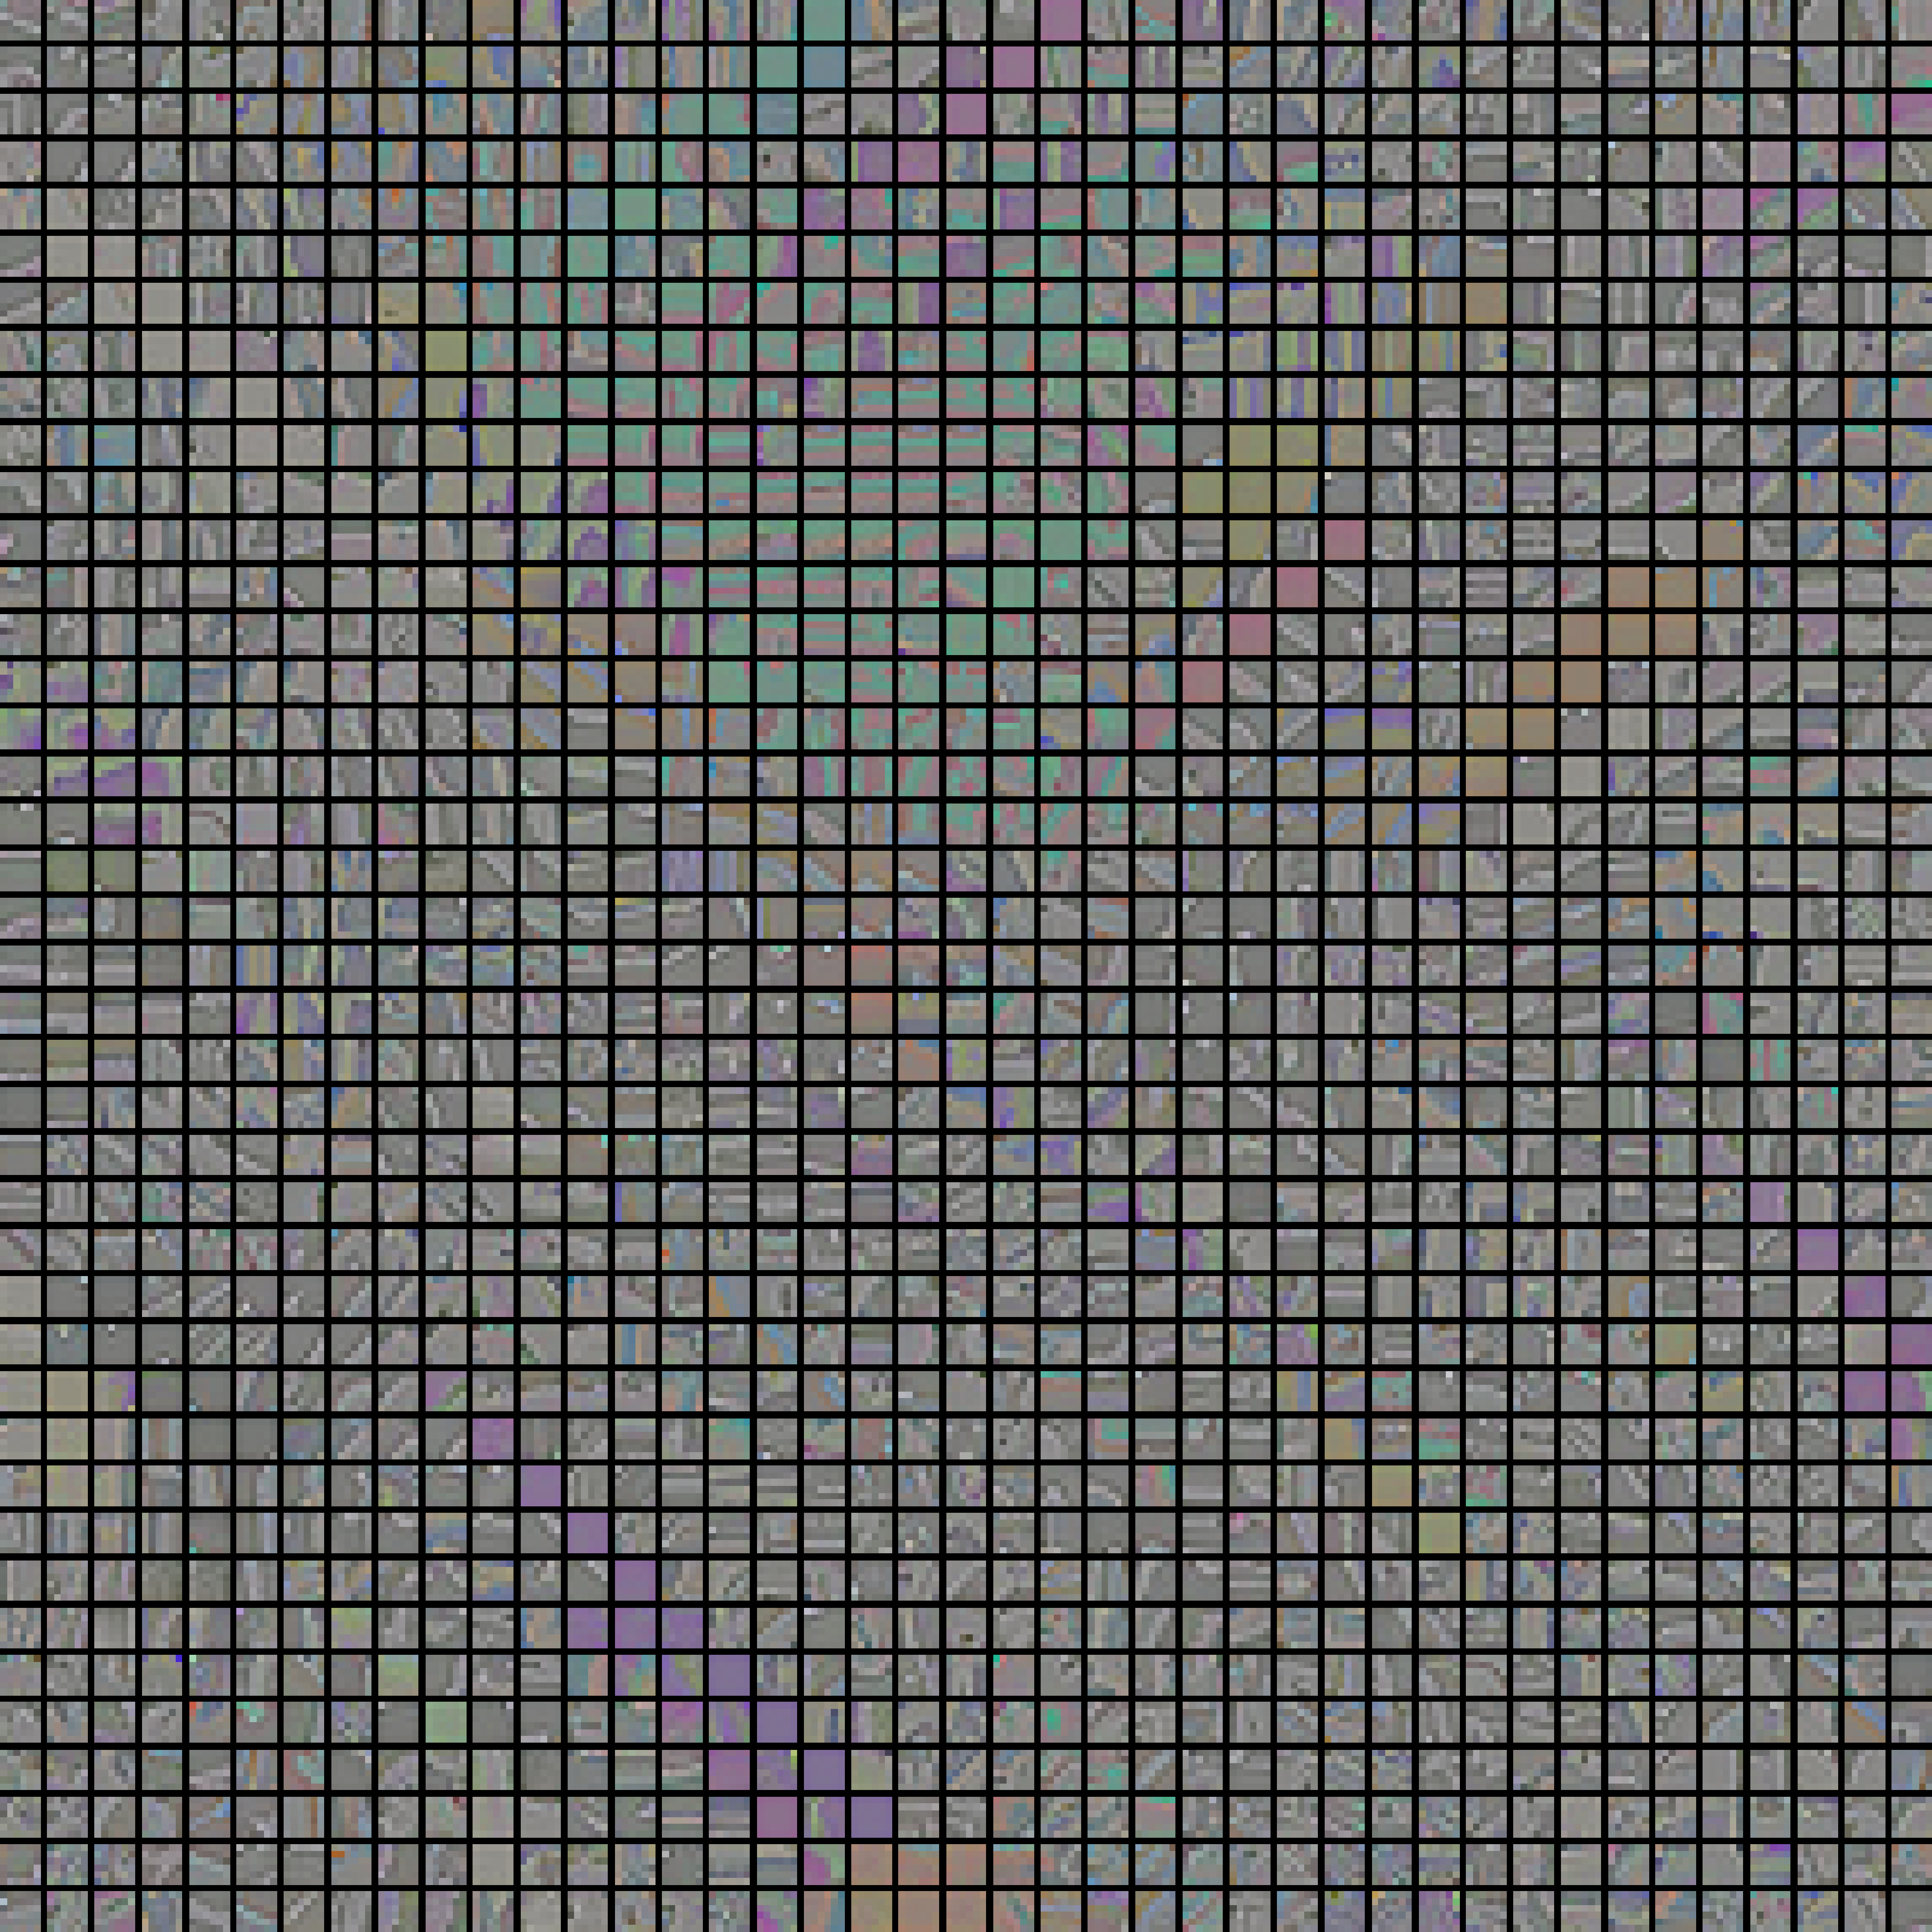
\includegraphics[width=0.5\linewidth]{figures/topographical_order_more_patches}
  \caption{An example of whitened dictionary  $\mathcal{D}$ from ImageNet-128 (Left), ImageNet-64 (Top-Right), CIFAR-10 (Bottom-Right). The atoms have been reordered via a topographic algorithm.\label{dico}}
\end{figure}

Once the dictionary $\mathcal{D}$ is fixed, for each patch $p_{i,x}$ we consider the following set of euclidean pairwise distances:
\begin{align*}\mathcal{C}_{i, x} =\{\Vert p_{i, x} - d \Vert\,, d\in\mathcal{D} \}\,.\end{align*}
 
For each whitened patch we encode the $K$ nearest neighbors of $p_{i,x}$ from the set $\mathcal{D}$, for some $ K \in \mathbb{N}$, which is a Vector Quantization (VQ) step.
More formally, we consider $\tau_{i,x}$ the $K$-th smallest  element of $\mathcal{C}_{i,x}$, and we define the $K$-nearest neighbors binary encoding as follow, for $(d,i)\in\mathcal{D}\times\mathcal{I}$:


\begin{equation}
\phi(x)_{d,i}=
\begin{cases}
1,&\text{if } \Vert  p_{i,x} - d\Vert \leq \tau_{i,x}\\
0,&\text{otherwise}.
\end{cases}
\end{equation}






Observe that this operation produces an output similar to the forward of a 1-hidden layer neural network, except that the non-linearity is not point-wise. In order to reduce the computational burdering of our method, we perform an intermediary average-pooling step.
Indeed, we subdivide $\mathcal{I}$ in squared overlapping regions $\mathcal{I}_k\subset\mathcal{I}$, leading to the representation $\Phi$ defined, for $d\in\mathcal{D}, k$ by:
\begin{align*}\Phi(x)_{d,k}= \sum_{i\in \mathcal{I}_k}\phi(x)_{d,i}\,.\end{align*}

The next section describes our classification pipeline, as we feed our representation $\Phi$ to a linear classifier on challenging datasets. Note that given the intermediary VQ, it would not be possible to learn the parameters of our dictionary via a standard differentiable method, consequently this approach fails to be analyzed directly through the scope of \cite{chizat2018global} for instance.




\section{Experiments}
\label{experiments}
We train  shallow classifiers (e.g., Linear and 1-hidden layer CNNs) on top of our reprensentation $\Phi$ on two widely used image classification datasets,  CIFAR-10 and ImageNet, which consist respectively of $5\times10^5$ small and $1.2\times10^6$ large color images  divided respectively in 10 and $10^3$ classes.


In each experiments, we employ 2D batch normalization in order to standardize our features on the fly. The spatial subdivision $\mathcal{I}_k$ are implemented as an average pooling with kernel size $n_1$ and stride $s$. 
As  $\Phi$ is high-dimensional, we factorize our linear classifier into a convolutional layer, a global average pooling and a final fully connected layer. This is motivated by similar considerations as the introduction of a "bottleneck" \cite{ResNet}. We apply a first convolutional layer that consists in $n_2$ convolution with stride 1 that reduces the number of channels from $\mathcal{D}$ to $c$. This reduces both the number of computations and the number of parameters, and this approach is well motivated by the natural translation invariance of images.

In all our experiments, we trained our linear classifier via SGD with momentum of 0.9, no weight decay and a fixed schedule for the learning rate, with the standard cross-entropy loss. We employed a standard data augmentation, however, we reduced the image resolution for ImageNet, which we discuss below.



\subsection{CIFAR-10}

 \paragraph{Implementation details}Since CIFAR-10 is small enough, we can use a "large" number of patches in the dictionary, i.e. up to $|\mathcal{D}|=1.6\times10^5$ patches with $Q = 6$.
The average pooling performed to reduce the size of the representation if of size $5$ and stride $3$. \Edouard{For the linear experiments, the linear layer hyperparameters are such that: $n_1=5, n_2=6,s=3,c=128$. For the 1-hidden layer experiment, we use: XXX}.
Our data augmentation consists in random crops of size $32^2$ after  padding of our images with $4$ pixels.

The $1 \times 1$ convolutional operator $C_1$ outputs $128$ channels.
The convolutional operator has a spatial size $6 \times 6$.
For the experiments with respectively $|\mathcal{D}|=2\times 10^3$ and $|\mathcal{D}|=1.6\times 10^5$ patches, we used respectively an initial learning of 0.003 and 0.001 that we decayed by 10 at respectively epochs 50,75 and 100, 150. This is consistent with standard renormalization when increasing the number of parameters \cite{trouver une citation, on dirait un sqrt(10) facteur qui indique la loss a pas été renormalisé, à vérifier}.


\paragraph{Classification experiments} Despite the relative simplicity of the encoding, our method performs comparably to other shallow methods with a linear classifier.
Compare to \cite{recht2019imagenet},  we use a much smaller number of patches ($16.000$ vs. $256.000$) for the same accuracy, and compare to \cite{mairal2016end}, we use an encoding of depth 1 without subspace learning (see \cite{mairal2016end} for details).
Using a 1 hidden layer classifier, the accuracy increases to $88.0 \%$ approaching the accuracy obtained with deep kernel methods \citep{li2019enhanced,shankar2020neural} and deep convoluitonal networks \citep{krizhevsky2012imagenet}.



\begin{table}[h]
  \caption{Accuracies on CIFAR-10}
  \label{accuracy}
  \centering
  \begin{tabular}{|c|c|c|c|c|c|c|c|}
    \hline 
    Reference&Name&$|\mathcal{D}|$&VQ&$Q$&Depth &Classifier& Acc. \\
    \hline 
    \hline 
    Ours&Patch&$10^3$ & Yes&6&1&linear&82.5 \\
    \hdashline[0.5pt/1pt]
    Ours&Patch&$10^4$ & Yes&6&1&linear&85.6\\
    \hdashline[0.5pt/1pt]
    \cite{coates2011analysis}&Dict.&$10^3$& Yes&6 & 1&linear & 68.6\\
    \hline 
    \cite{recht2019imagenet}&Dict.&$10^5$ & No& 6&1&linear &85.6\\
    \hdashline[0.5pt/1pt]
    \cite{mairal2016end}&CKN&$10^3, 10^4$& No&3 & 2& linear &85.8\\
    \hline
        
    Ours&Patch&$10^3$ & Yes& 6&2&1-NN&88.0\\
    \hdashline[0.5pt/1pt
     \cite{Oyallon_2015_CVPR}&Scatt.& - & No& 8 &2 & kernel & 82.3\\
     
    \hdashline[0.5pt/1pt]
    \cite{shankar2020neural}&CKN&-& No&3&5&kernel &89.8\\
        \hdashline[0.5pt/1pt]
    \cite{li2019enhanced}&NTK&$10^3$& No&6&6&kernel &88.9\\
    \hdashline[0.5pt/1pt]
    \cite{krizhevsky2012imagenet}&AlexNet&-& No&-&5&end-to-end&89\\
    \hline
  \end{tabular}
\end{table}




\begin{figure} 
  \label{fig:ablation_study}
  \centering
   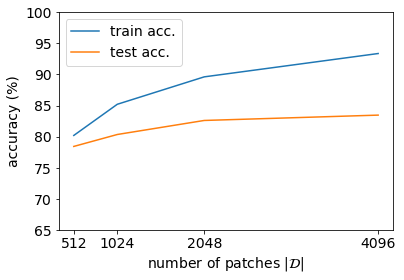
\includegraphics[width=0.3\linewidth]{figures/albation_study_npatches.png}
  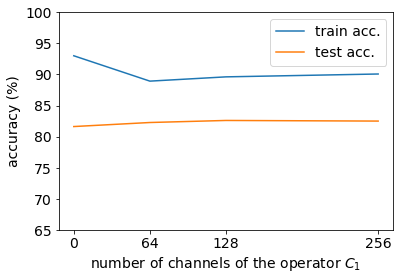
\includegraphics[width=0.3\linewidth]{figures/albation_study_classifier.png}
  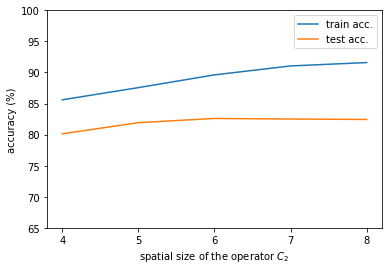
\includegraphics[width=0.3\linewidth]{figures/albation_study_classifier_2.png}
  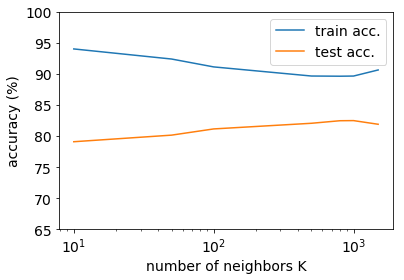
\includegraphics[width=0.3\linewidth]{figures/albation_study_K.png}
  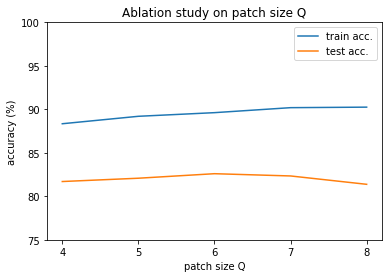
\includegraphics[width=0.3\linewidth]{figures/albation_study_Q.png}
  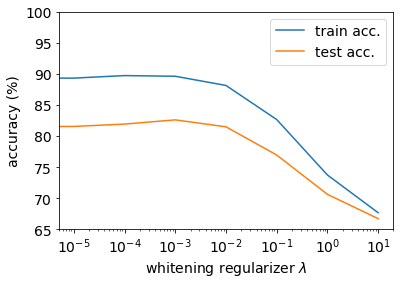
\includegraphics[width=0.3\linewidth]{figures/albation_study_lambda.png}\\
  \caption{CIFAR-10 ablation experiments on the number of patches  $|\mathcal{D}|$ (Top-left), the patch size $Q$ (Top-middle), the number of neighbors $K$ (Top-right), the whitening regularizer $\lambda$ (Bottom-left), and the number of channels of the factorized classifier(Bottom right).}
\end{figure}




\paragraph{Ablation experiments}
We decided to use CIFAR-10 to perform several ablation experiments because the experiments take substentially less time than on ImageNet. To measure the importance of different parameter choices, we perform an ablation study on the number of patches in the dictionary $|\mathcal{D}|$, the patch size $Q$, the number of neighbors $K$, the whitening regularizer $\epsilon$ and the number of channels $M$ of the factorized classifier.

The starting experiement uses  $|\mathcal{D}|=2048$ patches, a patch size $Q=6$, the number of neighbors $K=0.4\times 2048 = 820$, the whitening regularizer $\epsilon=1e-3$ and factorized classifier has $M=128$ channels.
Note that our representation is absolutely not sparse.


The number of patches $|\mathcal{D}|$ varies in $\lbrace 512, 1024, 2048, 4096 \rbrace$, the patch size $Q=6$ varies in $\lbrace 4, 5, 6, 7, 8 \rbrace$, the number of neighbors $K=$ varies in $\lbrace 10, 50, 100, 500, 800, 1000, 1500 \rbrace$, the whitening regularizer varies in $\lbrace0, 10^{-5}, 10^{-4}, 10^{-3}, 10^{-2}, 10^{-1}\rbrace$, the number of channels $c$ of the classifier varies in $\lbrace 0, 64, 128 ,256 \rbrace$, $0$ meaning that the classifier is not factorized, i.e. it is a standard fully connected linear operator, and the size of the convolution in the classifier varies in $\lbrace 4, 5 , 6, 7, 8\rbrace$
Results are shown in figure \ref{fig:ablation_study}.

One can see that the accuracy increases whith the number of patches of the dictionary.
The choice of the classifiier doesn't affect much the perfomance.
Unsprisingly, a fully connected classifier overfits more than a factorized classifier.
The accuracy is not very sentitive to the number of neighbors.
A small number of neighbors leads to large overfitting.
The optimum seem to be around $10^3$ neighbors, i.e. half of the number of patches in the dictionary.
The optimal patch size is $6$ but the accuracy for the other values is similar, and larger patches lead to overfitting.
Suprisingly, the whitening regularization $\lambda$ is not crucial as setting it to $0$ leads a $1\%$ drop in perfomance.
Large values of $\lambda$ tend to cancel the whitening effect since the term $\lambda I$ dominates $\Sigma$ in the whitening operator $W = (\lambda I+\Sigma)^{-1/2}$.
The accuracy drops severely for large values of $\lambda$, indicating that whitening is a key aspect of the representation.

\paragraph{Random filters and whitening} We note that whitening of patches is a systematic pre-processing step followed by the works cited in \cite{}.
Removing the whitening step leads to a drop in accuracy of about 17\%.
Using standardized Gaussian features leads to a drop in accuracy of about XX\%. This shows that this step is crucial for performance.


\begin{figure}
  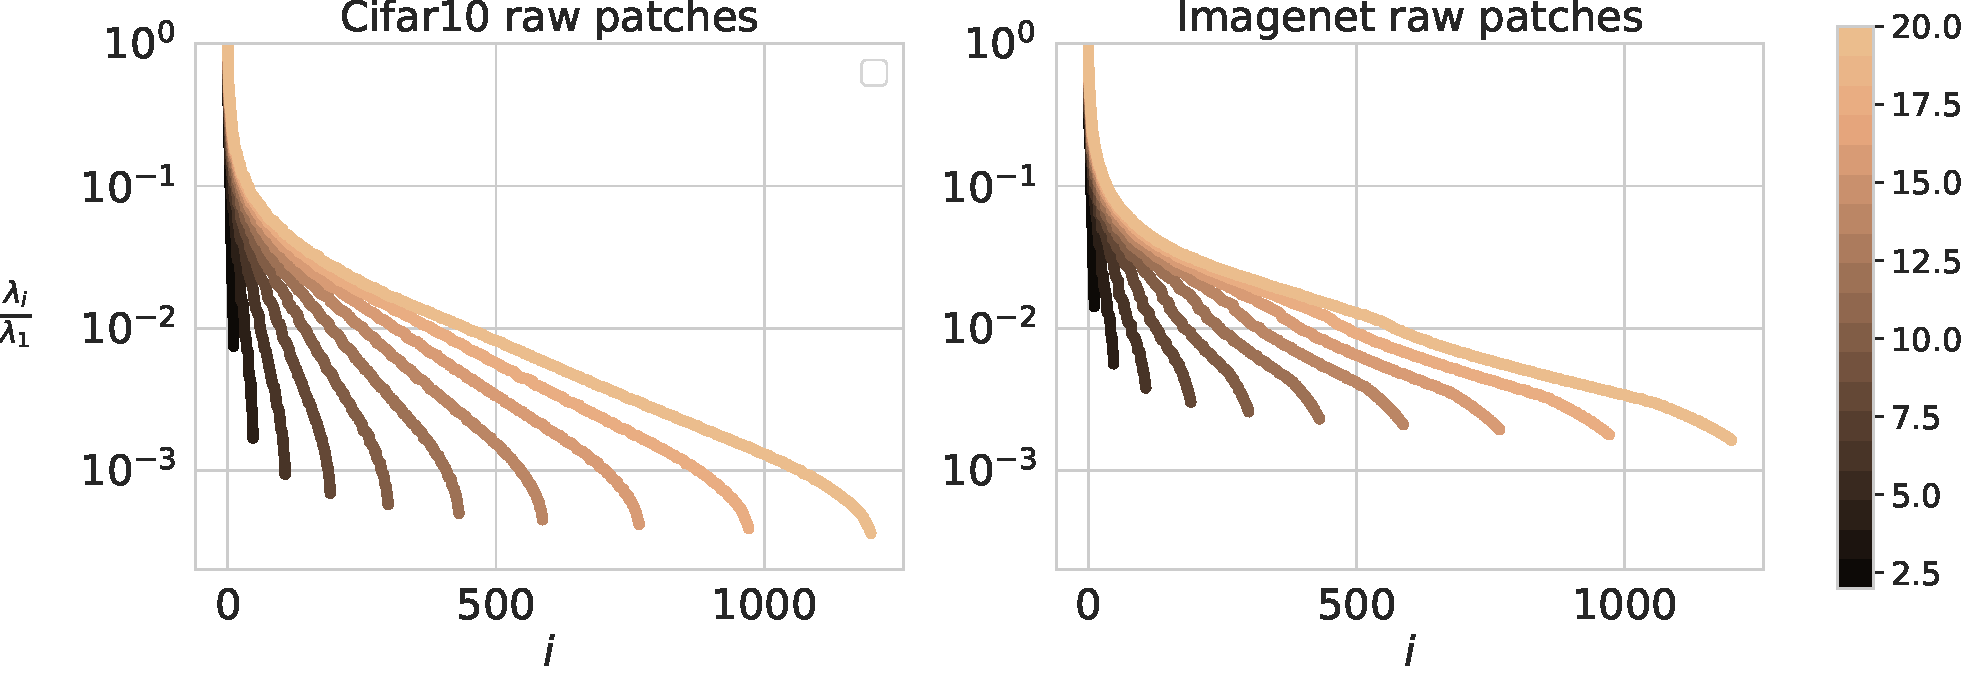
\includegraphics[width=1.\linewidth]{figures/spectrum_patches}
  \caption{Spectrum of $(\lambda \mathbf{I}+\Sigma)^{1/2}$ on CIFAR-10 (Left) and ImageNet-64 (Right).\label{dico}}
\end{figure}
\subsection{Imagenet}

\paragraph{Implementation details, ImageNet-64}  Since Imagenet is a much larger dataset than CIFAR-10, we limit ourselves to a number of patches up to $2048$. Here, $Q=6, n_1=, s=3$For reducing the computational overhead of our method on ImageNet, we employ lower-resolution images: we use $64^2$ and $128^2$ downsampled iamges using the "box" interpolation method, instead of the standard 224 length.  \cite{DBLP:journals/corr/ChrabaszczLH17} observed that this does not alterate much the top-performances of standard models ($-5 \%$ accuracy on average), and we also believe it introduces a useful dimensionality reduction, as it removes high-frequency part of images that are unstable \citet{chjdq}.

\paragraph{Implementation details, ImageNet-128}

\paragraph{Classification experiment}
The patch size $Q$ is $6$ for Imagenet64 and $12$ for Imagenet128.
The average pooling performed to reduce the size of the representation has  size $5$ and stride $3$ for Imagenet64 and size $10$ and stride $6$ for Imagenet128.
For training, we add a reflect padding of size $8$ for $64^2$ images and $16$ for $128^2$ images, and select a random crop of size $64^2$ or $128^2$.
We do not  modify the images for testing.
Note thas this procedure differs from the standard data-augmentation, which consists in resizing the smallest size of the image to a given size with constant image ratio, and selecting then a random crop for training and a center crop for testing.

The $1 \times 1$ convolutional operator $C_1$ outputs $256$ channels.
The convolutional operator $C_2$ has a spatial size $12 \times 12$.
We run the optimization during 60 epochs with an initial learning rate of 0.003 decayed by a factor 10 at epochs 40 and 50.

Eventhough it uses "low" image resolution ($64^2$), our method performs better than the  Scattering transform, state of the art method in unsupervised visual representation without representation learning (26.1 \% top1).
It outperforms some of seminal works on self-supervised deep representation learing methods like Look, Listen and Learn \citep{arandjelovic2017look} (32.3 \% top1), but the perfomance is far from recent self-supervised deep representation learing methods such as momentum-constrast (68.6 \% top1, \citep{he2019momentum} ) and contrastive predictive coding (71.5 \% top1, \citep{henaff2019data}).

Bagnets \citep{brendel2019approximating} have shown that a close to state of the art classification accuracy can be obtained with 50 layers convolutional networks that encode small patch information (patches of size $17^2$ or $33^2$ in $224^2$ images).
The perfomance obtained by our shallow encoding of the image patches neighborhood is a first step towards understanding the performance obtained by sophisticated patch encoding such as the Bagnets.
 
Increasing the size of the resolution and the size of patches from $64$ and $6$ to $128$ and $12$ improves the performance, showing that the nearest neighbors are still meaningfull in the space of patches of size $12$.
These patches are in a space of dimension $12^2 \times 3 = 432$, but distance to nearest neighbors are know to be meaningless in uniformly distributed spaces of dimension $10 -15$ \citep{beyer1999nearest}.
This shows a form of low-dimensionalty in the natural image patches.


\begin{figure}
	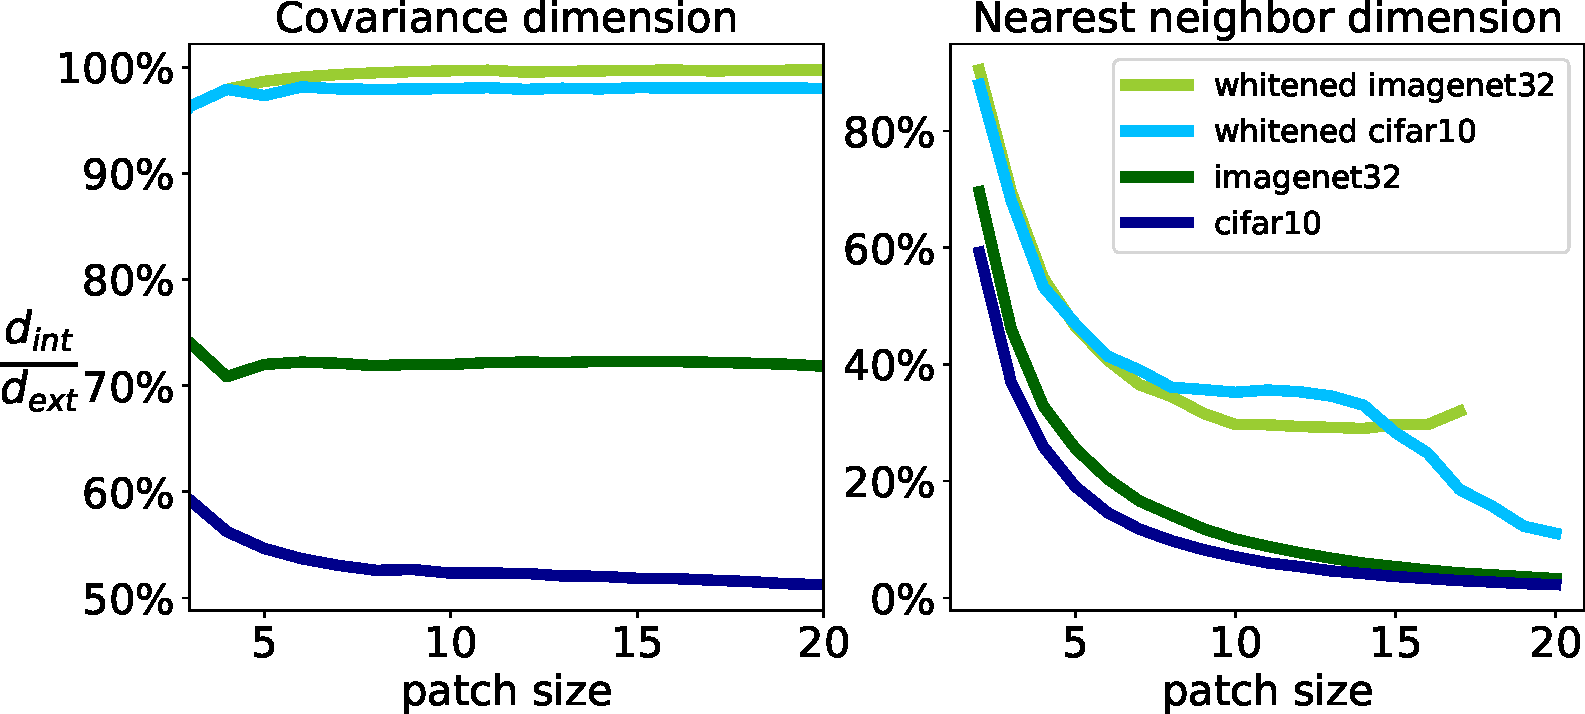
\includegraphics[width=.95\linewidth]{figures/intrinsic_dims}
	\caption{(Left) Ratio between covariance dimension and extrinsic dimension of the patches as a functions of their size. (Right) Ratio between nearest neighbor dimension and extrinsic dimension of the patches as a functions of their size.}
\end{figure}
\paragraph{Random filters and whitening}


\begin{table}[h]
  \caption{Accuracies on ImageNet}
  \label{accuracy}
  \centering
  \begin{tabular}{|c|c|c|c|c|c|c|c|c|}
    \hline 
    Reference&Name& $|\mathcal{D}|$ & $Q$ & Depth & Res. & Classifier & Top-1&Top-5 \\
    \hline 
    \hline
    Ours&Patch&2048 & 6 & 1 & 64 & linear & 33.4 &  54.7 \\
    \hdashline[0.5pt/1pt]
    Ours [runnning] &Patch&2048 & 12 & 1 & 128 & linear & 31.2  &  52.4 \\
    \hdashline[0.5pt/1pt]
    \cite{zarka2019deep}&Scatt. & - & 32 & 2 & 224 & linear & 26.1  & 44.1 \\
    \hdashline[0.5pt/1pt]
    \cite{arandjelovic2017look}&Random CNN & - & - & 9 & 224 & linear & 18.9  & N.C.\\
    \hline
    \cite{arandjelovic2017look}&Look, Listen, Learn & - & - & 9 & 224 & linear & 32.3   & N.C.\\
     \hdashline[0.5pt/1pt]
    \cite{sanchez2013image} & FV& - & 24 & 3 & full& linear & N.C. & 72.0\\
    \hline
     Ours [runnning]&Patch&2048 & 6 & 2 & 64 & 1-NN & 36.4 &  58.0 \\
     \hdashline[0.5pt/1pt]
   \cite{brendel2019approximating} & BagNet & - & 33 & 50 & 224 & end-to-end & N.C. & 87.6
    \\
    \hdashline[0.5pt/1pt]
   \cite{}&shallow 1-hidden layer&-&-&1&224&end-to-end&&\\
    \hdashline[0.5pt/1pt]
   \cite{}&shallow 2-hidden layer&-&-&2&224&layerwise&&\\
    \hdashline[0.5pt/1pt]
    & AlexNet&&&&&&&\\
   \hline
  \end{tabular}
\end{table}








\paragraph{VQ and soften non-linearity}
\subsection{Dictionary structure}
\paragraph{Comparison between the patches of CIFAR and ImageNet} In Fig. \label{spectrum}, we display the spectrum of...
\paragraph{Spectrum of $\mathcal{D}$}
\paragraph{Intrinsic dimension of $\mathcal{D}$}
\section{Conclusion}
parler du unforgettable je sais pas quoi



\bibliographystyle{abbrvnat}
\bibliography{biblio}{}

\newpage

\appendix

\section{Mahanalobis distance and whitening}

The Mahalanobis distance \citep{chandra1936generalised, mclachlan1999mahalanobis} between two samples $x$ and $x'$ drawn from a random vector $X$ with covariance $\Sigma$ is defined as  
\begin{align*} D_M (x, x' ) =  \sqrt{ (x - x')^T \Sigma^{-1} (x - x')} \end{align*}
If the random vector $X$ has identity covariance, it is simply the usual euclidian distance :
\begin{align*} D_M (x, x' ) =  \| x - x' \| \end{align*}

Using the diagonalization of the coraviance matrix,  $\Sigma = P\Lambda P^T$, the affine whitening operators of the random vector $\mathbf{X}$ are the operators 
\begin{equation}
\label{whitening}
     w : \mathbf{X} \mapsto O \Lambda^{-1/2} P^T (\mathbf{X} - \mu), \quad \forall O \in  O_n (\mathbb{R})
\end{equation}
For all whitening operator $w$ we have :
\begin{align*}
\|w(x) - w(x')\| = D_M(x, x')
\end{align*}
Indeed 
\begin{align*}
  \|w(x) - w(x')\|
    &= \| O \Lambda^{-1/2} P^T ( x - x') \|\\
    &= \sqrt{(x - x')^T P \Lambda^{-1/2} O^T O \Lambda^{-1/2} P^T (x - x') }\\
    &=  \sqrt{ (x - x')^T P \Lambda^{-1} P^T (x - x')} \\
    &= D_M(x, x') 
\end{align*}

\section{Implementation of the K nearest neighbors as a 1 layer convolutional network}

In this section, we explicitely write the whitened patches with the whitening operator $W$.
Recall that  we consider the following set of euclidean pairwise distances:
\begin{align*}\mathcal{C}_{i, x} =\{\Vert W p_{i, x} - W d \Vert\, d\in\mathcal{D} \}\,.\end{align*}

For each image patch we encode the $K$ nearest neighbors of $W p_{i,x}$ in the set $Wd, d \in \mathcal{D}$, for some $ K \in 1 \ldots|\mathcal{D}| $.

Using the square distance instead of the distance doesn't change the $K$ nearest neighbors.
We have 
\begin{align*} \Vert Wp_{i,x} - Wd \Vert^2 = \Vert Wp_{i,x} \Vert^2 - 2 \langle p_{i,x}, W^T W d \rangle + \Vert Wd\|^2 \end{align*}
The term $\|Wp_{i,x}\|^2$ doesn't affect the $K$ nearest neighbors, so the $K$ nearest neighbors are the $K$ smallest values in
\begin{align*}
        \|Wd \|^2 - 2\langle p_{i,x}, W^T W d \rangle
\end{align*}
or equivalently the  $K$ largest values in

\[
        \langle p_{i,x}, W^T W d \rangle - {\|Wd \|^2 \over 2} 
\]
This can be implemented in a convolution of the image using $W^T W d$ as filters and ${\|Wd \|^2 \over 2}$ as bias term, followed by a vectorwise non-linearity that binary encodes the $K$ largest values in the channel dimension.

To compute the $K$ nearest neighbors in $\mathcal{D}$ we have to compute the quantity
\begin{align*} \langle p_{i,x}, W^T W d \rangle - {\|Wd \|^2 \over 2} \end{align*}
We can then easily compute 
\begin{align*} - \langle p_{i,x}, W^T W d \rangle - {\|Wd \|^2 \over 2} \end{align*} which is the quantity needed to compute the $K$ nearest neighbors in the set of negative patches $\overline{\mathcal{D}}$.
This is a cheap way of doubling the number of patches.


\end{document}
